\cleardoublepage
\chapter{Introduction}
\label{ch:chapter1}


\section{Motivation and objectives}\label{sec:motivación-y-objetivos}

The \texit{Deep Learning}~\cite{deep_learning} area has advanced exponentially in the last years.
This has allowed to have predictive models capable of processing images and classifying them according to their primary features.
The main consequence of this process is the opening of a window of opportunity for the exploitation of these models in a real environment, with the objective of making them crucial when detecting fires, earthquakes, as well as all kinds of natural disasters.

The efficient use of these models requires an infrastructure capable of supporting the necessary reliability in terms of availability and speed.
In these cases, real-time processing becomes essential to optimize emergency resources, manage teams to the most affected disaster areas and prevent the maximum possible risks.


The points that resumes this project are: firstly, the acceleration of the training time of a \texit{Deep Learning} model using a GPU~\cite{gpu_solution}
in the Google Colab service, and secondly, optimization of model inference time using the Intel OpenVINO toolkit. Finally, the model will be deployed in a cloud environment where it can operate as a service capable of supporting thousands of concurrent calls.
TensorFlow~\cite{deep_learning_tensorflow}, an open source framework developed by Google for the preparation of neural network training algorithms, has been used as the main tool to carry out the model training.

With the requirement for the application to be maintainable and flexible to possible changes, Docker\footnote{\rule{https://www.docker.com/}} container technology has been used.
Using this tool ensures that the versions of the operating system and external libraries are compatible with each other, additionally, the possibility of porting the application to different environments that take advantage of this container solution is left open.
The achievement of general goals is carried out by following a series of specific objectives, which are listed below:
\begin{itemize}
    \item Improvement in the training times of a model of
    \texit{Deep Learning} using a GPU from the Google Colab service.
    \item Converting a TensorFlow model to an OpenVINO model to increase its inference speed.
    \item Preparation of a Google cloud architecture capable of supporting concurrent traffic in optimal times for the service.
    \item Coding of an application capable of making use of the different inference systems of TensorFlow and OpenVINO\@.
    \item Coding of a web application suitable to expose all services in a production environment.
    \item Encapsulation of the different environments using Docker.
    \item Application deployment and load tests.
    \item Obtaining results and performance comparing between the different inference systems, hardware and web servers.
\end{itemize}


\section{State of the art}\label{sec: state-of-the-art}
Currently, artificial intelligence is made up of several branches such as machine learning, natural language processing, among others. One of them is \texit{Deep Learning}.
The deep learning architecture pursues the study and classification of a variety of problems
making use of their own algorithms.
Currently, \texit{Deep Learning} algorithms are used for all kinds of problems that cover a multitude of sectors within the industry \cite{robotics}, governments and, ultimately, society itself. The digitization and expansion of the internet provides countless data sources capable of being processed and analyzed by this kind of algorithms, which are used for different purposes.


The source of the data has changed, now they come from interactions that users have with their mobile devices, calls, internet money transactions \cite{crypto}, navigation of web pages and, in the case of this project, images from a satellite.
Image processing has been an advance in society that police forces are now taking advantage of, using these tools to detect license plates or to recognize potential criminals\footnote{\url{https://www.nhtsa.gov/sites/nhtsa.dot.gov/files/documents/809811-lidarspeedmeasuringdevice.pdf}}; doctors, who use these systems \cite{medic} to improve the early detection of some types of cancer\footnote{\url{https://www.nature.com/articles/srep46450}}, or in the case of industry, which is helped by these solutions to automate and classify processes that previously involved the supervision or execution of a person.
In the same way, countries have their personal image recognition systems for classifying their citizens, recommendation systems both for companies seeking to increase their sales and for banks seeking loan-eligible individuals, and even to avoid undesirable content through the web.



In general, the massive amount of data has created a necessity for exploitation
through them, the \texit{Deep Learning} is positioned as a reliable tool to give value to all the interactions that are occurring almost permanently
in every technological system on the planet.
All this stimulus leads to the creation of thousands of new jobs in the technology sector, dedicated exclusively to the application of machine learning algorithms, as well as to the increase in their teaching.
This has opened the possibility for professionals who previously did not have a clearly defined role in this field to position themselves as practically indispensable.
The benefits are noticeable in studies like math, statistics, and related. In these areas, mathematical profile and analytical skills are highly valued for carrying out this type of task.


The development of this new profile of professionals has encouraged the use of less common programming languages. This is because its use and learning curve is more affordable than   other more traditional languages, in the case of Java or C++ (see Figure ~\ref{fig:Encuesta sobre lenguajes de programación en StackOverflow 2019}). Along with this, new free and open source \cite{open} tools have emerged, such as Jupyter, TensorFlow, Scikit-learn or PyTorch, among others.


\begin{figure}
    \centering
    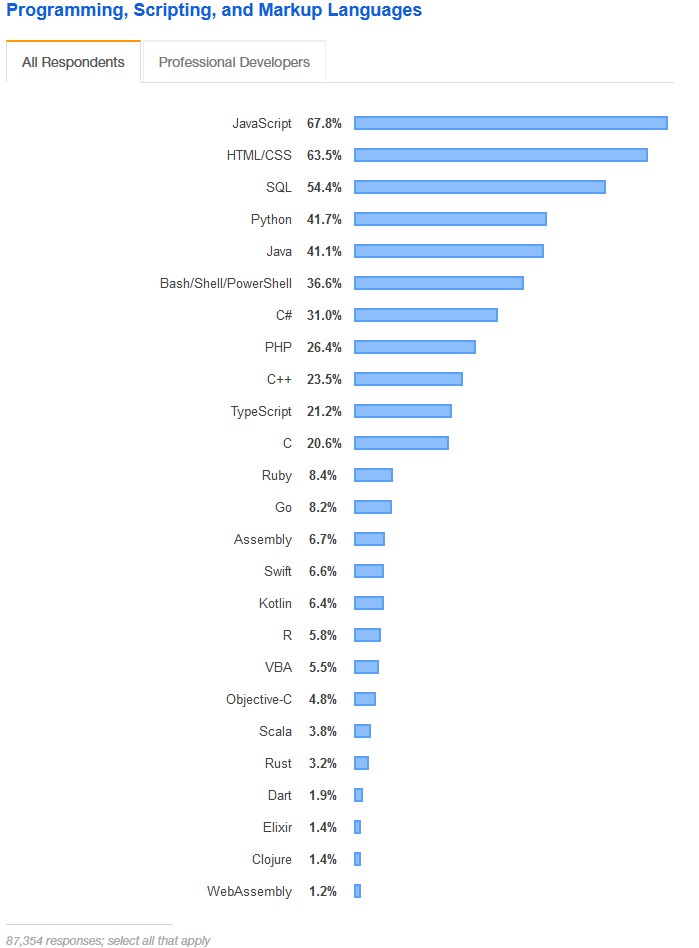
\includegraphics[width=0.95\textwidth]{images/chapter1/stackoverflow_language.png}
    \caption{Survey of programming languages at StackOverflow 2019.}
    \label{fig:Encuesta sobre lenguajes de programación en StackOverflow 2019}
\end{figure}

\subsection{Deep Learning concept}\label{subsec:concepto-deep-learning}

The \texit{Deep Learning} has its defining element the use of algorithms that base its structure on artificial neural networks, imitating the behavior of human beings and their central nervous system.
The strength provided by the emergence of Big Data has made this type of technology become the daily practice of many professionals.
One of the keys to the \texit{Deep Learning} algorithms is in the learning capacity that resides in them.
This gives us the ability to deal with real world problems,
where combinations of possibilities and pattern recognition are left out of our calculations.
Neural networks represent the main tool for classifying images. This is because they can extract fundamental characteristics from each pixel and have a high percentage of accuracy in the prediction.



In order to materialize all these machine learning algorithms we have services from large companies such as Google, Amazon, IBM, which
implement their own business solutions \cite{cloud_computing}.
But we can also choose open source tools like TensorFlow, one of the most famous \texit{Deep Learning} libraries developed by Google engineers, later released under Apache license.
We also have others like PyTorch and Keras.
All of the them were originally developed for the Python programming language, which has seen its usage percentage increase due to this machine learning \cite{python_machine} wave.


\subsection{Neural networks in image processing}\label{subsec: neural-networks-in-image-treatment}
The basic processing unit for neural networks is the perceptron (see Figure ~\ref{fig:Perceptrón}),
which develops an algorithm capable of generating selection criteria for subsets of neurons.
This set of neurons will become part of the different layers that completely compose the neural network.
Each neuron receives an input, either from an external source or from another neuron.



\begin{figure}[H]
    \centering
    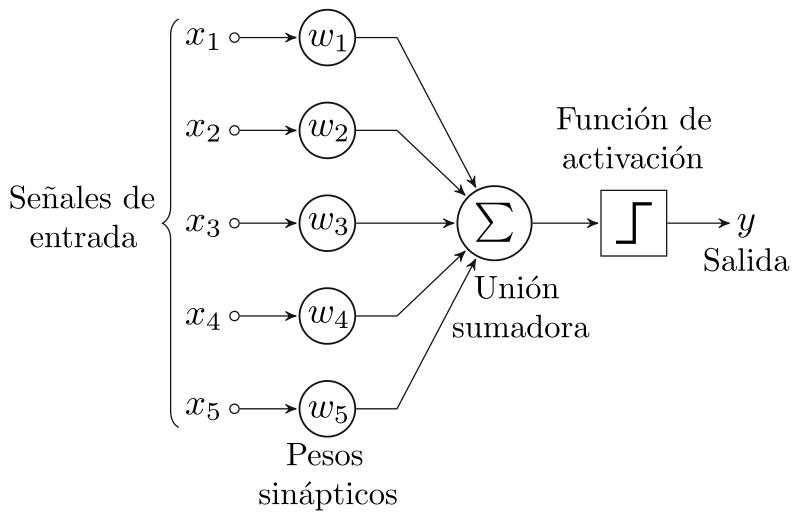
\includegraphics[width=0.6\textwidth]{images/chapter1/perceptron.png}
    \caption{Perceptron example.}
    \label{fig:Perceptrón}
\end{figure}

Each neuron applies a calculation function which generates the corresponding weights of each neuron. These weights represent the level of interaction of the neurons and should be adjusted so that they are as close as possible to the data we know.
The input weights of a layer originate from a previous layer, and its outputs are part of the input of a subsequent layer. Propagation occurs until we reach the last layer of the network, which will be the output layer from which we obtain the result of our classification.

In this specific problem, we focus on classifying multispectral images \cite{imageProcessing} with high spatial resolution using the RGB spectral bands (Red, Green and Blue).
Our set of images belongs to an area partially destroyed by a natural disaster in Haiti, which occurred in 2010.
These images were acquired by the GeoEye-1 high-resolution Earth observation satellite, launched in September 2008.
Therefore, the purpose of our \texit{Deep Learning} model is to have the ability to classify these images depending on whether the area is damaged or in good condition.

\section{Work plan}\label{sec: work-plan}
In Figure~\ref{fig:Plan de trabajo} we can see the plan for achieving the objectives followed in this work.
The effort metric that appears in it refers to the number of days invested in each task, with a total sum of 10 weeks.
The activities are sequentially ordered in their execution and have a dependency on each other, so it has never been
moved on to another task without completing the previous one.



\begin{figure}[H]
    \centering
    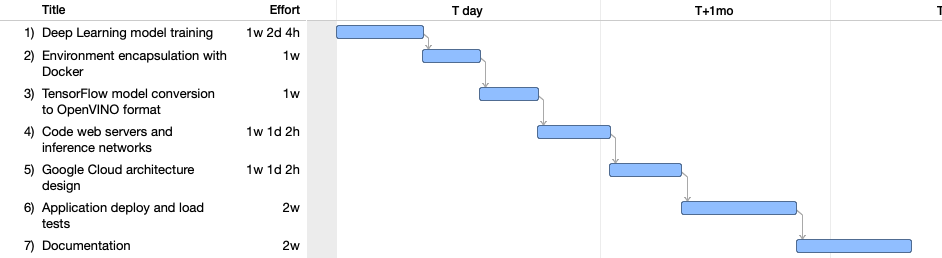
\includegraphics[width=1\textwidth]{images/chapter1/work_plan_eng.png}
    \caption{Work plan.}
    \label{fig:Plan de trabajo}
\end{figure}

\section{Organization of this project}\label{sec:organización-de-esta-memoria}

Bearing in mind the above specific objectives, we proceed to describe the organization of the rest of this project, structured in a series of chapters whose contents are
described below:

\begin{itemize}
    \item\textbf{Training the model using Google Colab}: The training and speed increase process using the Google Colab platform and its associated hardware.
    \item\textbf{OpenVINO technology}: The purpose of the Intel OpenVINO toolkit is defined, as well as the transformation of a TensorFlow model to be compatible with said solution.
    \item\textbf{Proposed Cloud Architecture}: Explanation of the Google Cloud architecture designed to support the entire application infrastructure.
    \item\textbf {Experimental results}: The different web frameworks to be tested using the Python programming language are prepared, showing the performance obtained in the training and inferences phases. In addition, the approximate calculation of the project costs will be presented.
    \item\textbf{Conclusions and future work}: The conclusions obtained through load tests and also some possible lines of future work.
\end{itemize}

